\section{Durchführung}
\label{sec:Durchführung}

Zuallererst wird der verwendete Selektivverstärker untersucht. Auf diesen wird
eine sinusförmige Wechselspannung gegeben. Mithilfe eines Millivoltmeters kann
die Ausgangsspannung $U_\text{a}$ abgelesen werden. Es wird nun die Ausgangsspannung
in Abhängigkeit der eingestellten Frequenz der eingehenden Wechselspannung gemessen
und notiert. Um das Maximum der Filterkurve herum werden mehr Messwerte aufgenommen als
an den Rändern.\\
In Abbildung \ref{fig:schaltung} ist die Schaltung der Messaparatur zu sehen.

\begin{figure}[H]
  \centering
  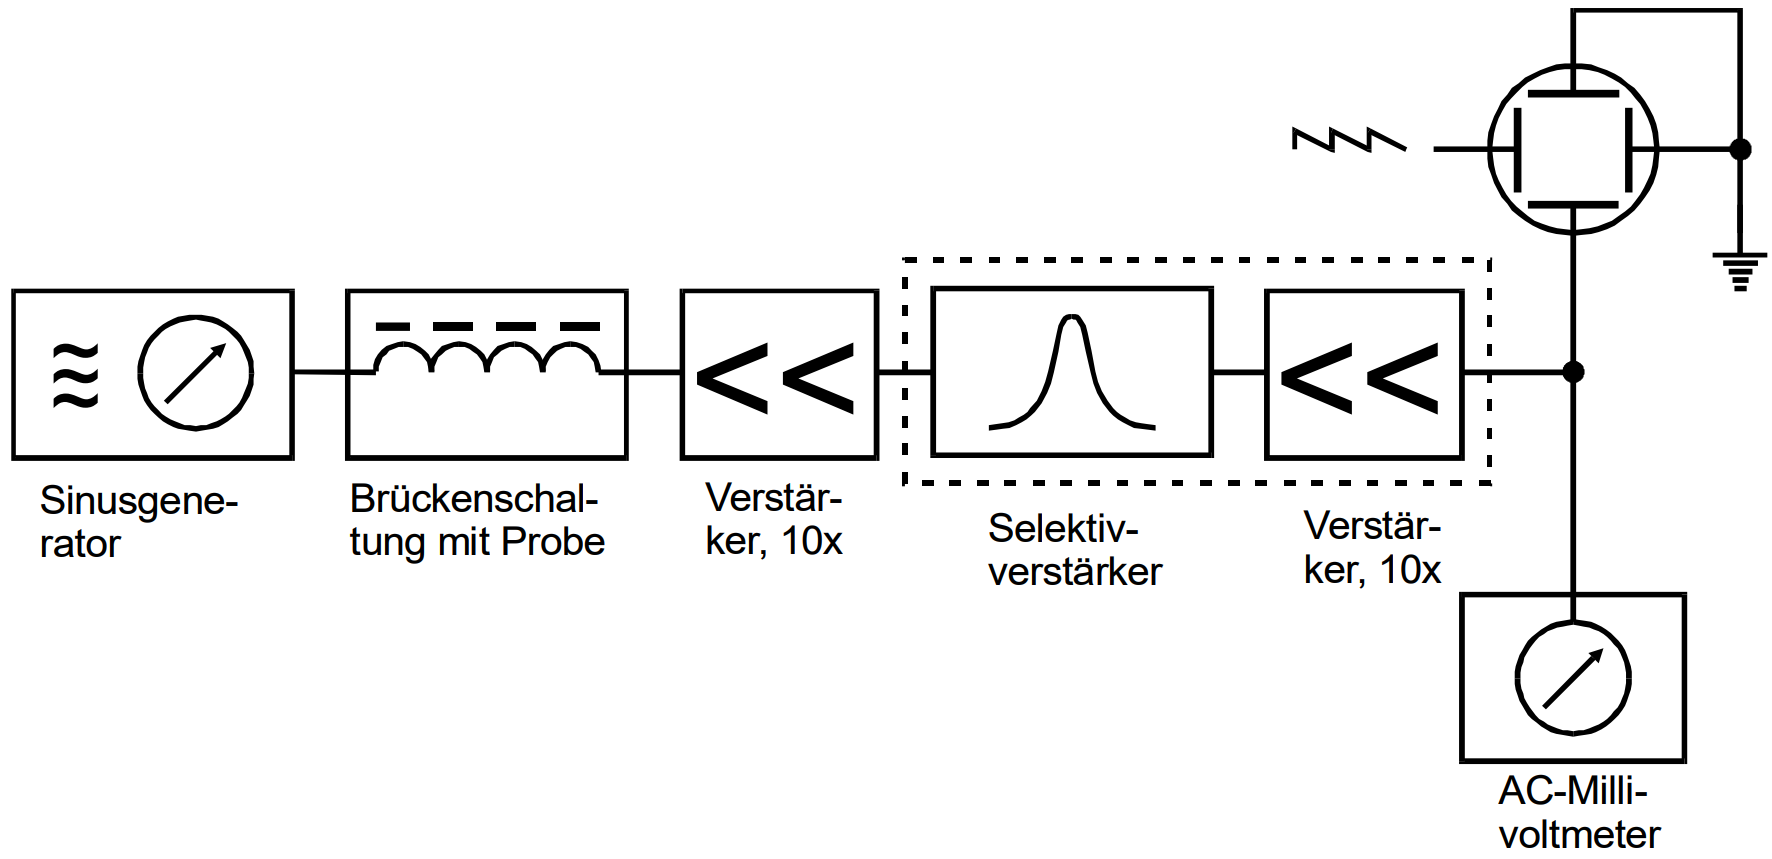
\includegraphics[width=250pt]{data/schaltung.png}
  \caption{Skizze zur Schaltung der verwendeten Messapparatur\cite{Versuchsanleitung}}
  \label{fig:schaltung}
\end{figure}

Es ist zu erkennen, dass der Selektivverstärker an die Brückenschaltung, skizziert in
Abbildung \ref{fig:brueckenschaltung}, angeschlossen wird. Erneut wird eine sinusförmige
Wechselspannung auf die Brückenschaltung gegeben. Mithilfe des Potentiometers wird die
Brückenspannung auf ein Minimum geregelt. Der Wert der Ausgangsspannung und der am Potentiometer
eingestellte Widerstand werden aufgezeichnet. Die Probe wird behutsam in die Spule eingeführt.
Die veränderte Ausgangsspannung wird notiert. Die Brückenspannung durch Einstellen
des Potentiometers erneut auf ein Minimum geregelt und der eingestellte Widerstand notiert.
Dieses Verfahren wird so für alle vier Proben wiederholt.
